\subsection{Features of Graphs Points, Domain, Range}
\begin{definition}[Graph Points]
	A graph point of a function is an ordered pair $(x, y)$ on a coordinate plane, where $y$ is the output generated when the function precesses the input $x$.
\end{definition}
\begin{example}[Graphs]
	\hfill
	\begin{center}
	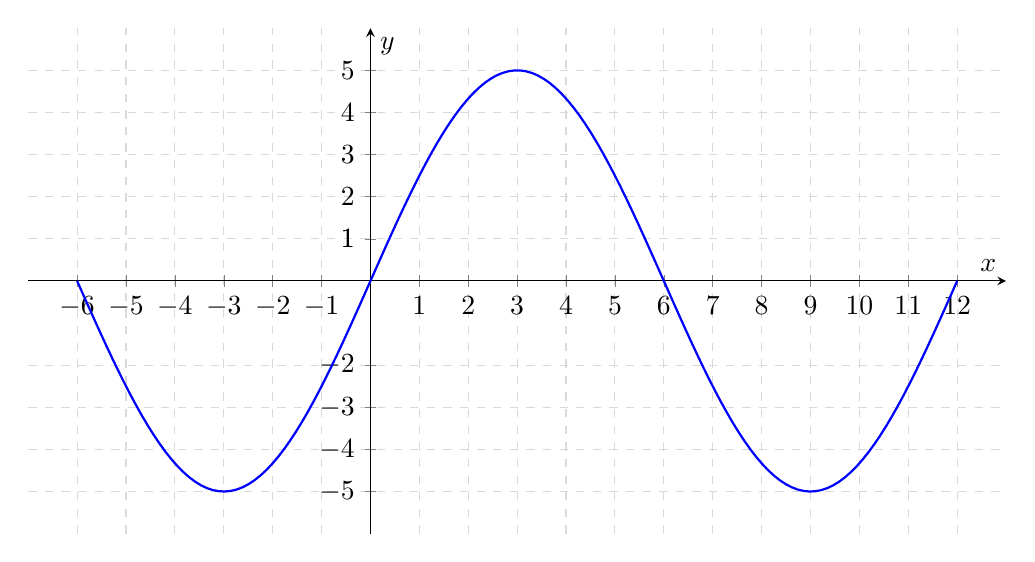
\begin{tikzpicture}
		\begin{axis}[
			width = 14cm,
			height = 8cm,
		    axis lines = middle,
		    xlabel = $x$,
		    ylabel = $y$,
		    xmin = -7, xmax = 13,
		    ymin = -6, ymax = 6,
			xtick = {-6, -5, -4, -3, -2, -1, 0, 1, 2, 3, 4, 5, 6, 7, 8, 9, 10, 11, 12},
			ytick = {-5, -4, -3, -2, 1, 0, 1, 2, 3, 4, 5},
		    grid = both,
		    grid style = {dashed, gray!30}
		]
		    \addplot [domain=-6:12, samples=150, thick, blue] {5*sin(30*x)};
		\end{axis}
	\end{tikzpicture}
	\end{center}
	\begin{enumerate}
		\item Find $f(0) = 0 \quad (0, 0)$
		\item Find $f(-2) = -2 \quad (-2, -2)$
		\item Is $f(1) \, positive \lor \, negative \, = \, positive$
		\item Is $f(-2) \, positive \lor \, negative \, = \, negative$
		\item For what $x$ is $f(x) = 0$? \\
		$(-6, 0)\, (0, 0)\, (6, 0)\, (12, 0) \quad x = -6,\, 0,\, 6,\, 12$
		\item For what $x$ is $f(x) > 0$? \\
		$0 < x < 6 \quad (-4, 6)$
		\item For what $x$ is $f(x) < 0$? \\
		$-6 < x < 0,\, 6 < x < 12 \quad (-6, 0) \cup (6, 12)$
		\item Domain: $D : \{x \mid -6 \le x \le 12\} \quad [-6, 12]$
		\item Range: $R : \{f(x)  \mid -5 \le f(x) \le 5\} \quad [-5, 5]$
		\item $x$ Intercept: $(-6, 0), \, (0, 0), \, (6, 0), \, (12, 0)$
		\item $y$ intercept: $(0, 0)$
		\item How many times does the $y = 2$ cross the graph? $2$
		\item For what $x$ is $f(x) = 4$? \\
		$(2, 4)\, (4, 4)$
		\item For what $x$ is $f(x) = -5$? \\
		$(-3, -5)\, (9, -5)$
	\end{enumerate}
\end{example}

\begin{definition}[Square Brackets: Inclusive]
	``[`` or ``]`` The endpoint number is included in the interval (corresponds to $\le \lor \ge$).
\end{definition}

\begin{definition}[Parentheses: Exclusive]
	``(`` or ``)`` The endpoint number is not included in the interval (corresponds to $< \lor >$). It is also always used for infinity ($\infty$).
\end{definition}

\begin{example}[Algebraic]
	$$f(x) = \frac{x + 2}{x - 6}$$
	\begin{enumerate}
		\item $f(1) = \frac{(1) + 2}{(1)- 6} \to \frac{3}{5} \quad \left(1, -\frac{3}{5}\right)$
		\item $f(x) = 2$ ... find $x$\\
		$2 = \frac{x + 2}{x - 6}$ \\
		$2x - 12 = x + 2$ \\
		$x - 12 = 2$ \\
		$x = 14$ \\
		$(14, 2)$
		\item Domain: \\
		$x - 6 = 0$ \\
		$x = 6$\\
		$D = \{x \mid x \ne 6\}$ \\
		$(-\infty, 6) \cup (6, \infty)$
		\item $x$ intercept:
		$f(x) = 0$ \\
		$0 = \frac{x + 2}{x - 6}$ \\
		$x + 2 = 0$ \\
		$x = -2$ \\
		$(-2, 0)$
		\item $y$ intercept: \\
		$f(0) = \frac{(0) + 2}{(0) - 6} = -\frac{1}{3}$ \\
		$\left(0, -\frac{1}{3}\right)$
	\end{enumerate}
\end{example}
